\chapter{Methods}

Let us get to the core of this work. In this chapter, I'll first describe the dataset on which the individual models are evaluated. For a more detailed problem description, see ~\ref{Protein_description}. With the data described, I'll show how the models interact with it.

\section{Datasets}

The datasets used in this work are for \ac{LBS} prediction. The motivation and chemical background for it are described in ~\ref{Protein_description}. Now, let us look into how the data is presented in the program and what preprocessing could be done with it.

\subsection{Raw data intuition}

The raw input into any of our models is the protein's 3D structure. This is represented by a SAS point cloud on the protein's surface. Each point has a feature vector attached, which represents the chemical properties of the given accessible surface patch. Each point also has an LBS class, which the model trains and predicts. These can be seen in the figure~\ref{fig:class_point_cloud}.

\begin{figure}
    \centering
    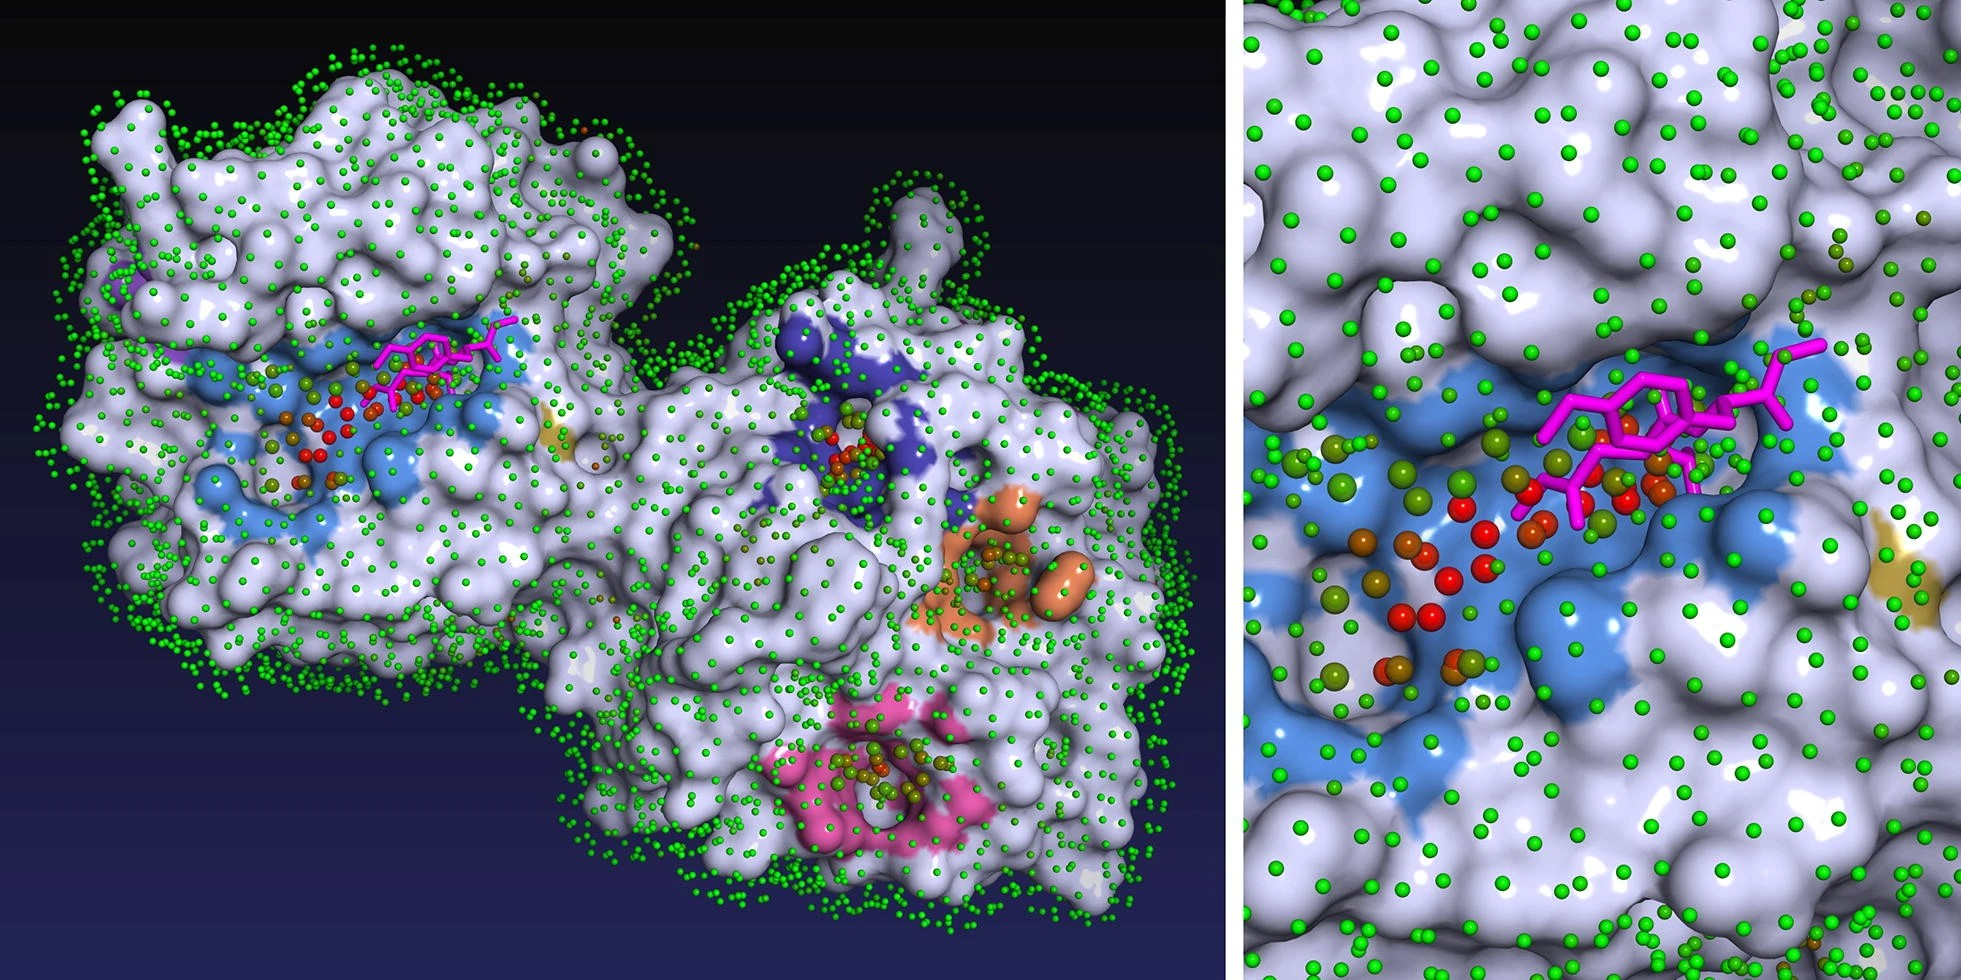
\includegraphics[width=0.5\linewidth]{p2rank.jpg}
    \caption{Visualization of a molecule taken directly from \cite{P2RANK}. The protein surface is covered by SAS points represented by green to red points representing predicted ligandability  (from 0 = green to 1 = red). The largest pocket (shown in the close-up) is indeed a correctly predicted true binding site that binds a known ligand (magenta).}
    \label{fig:p2rank_visualization}
\end{figure}

\begin{figure}
    \centering
    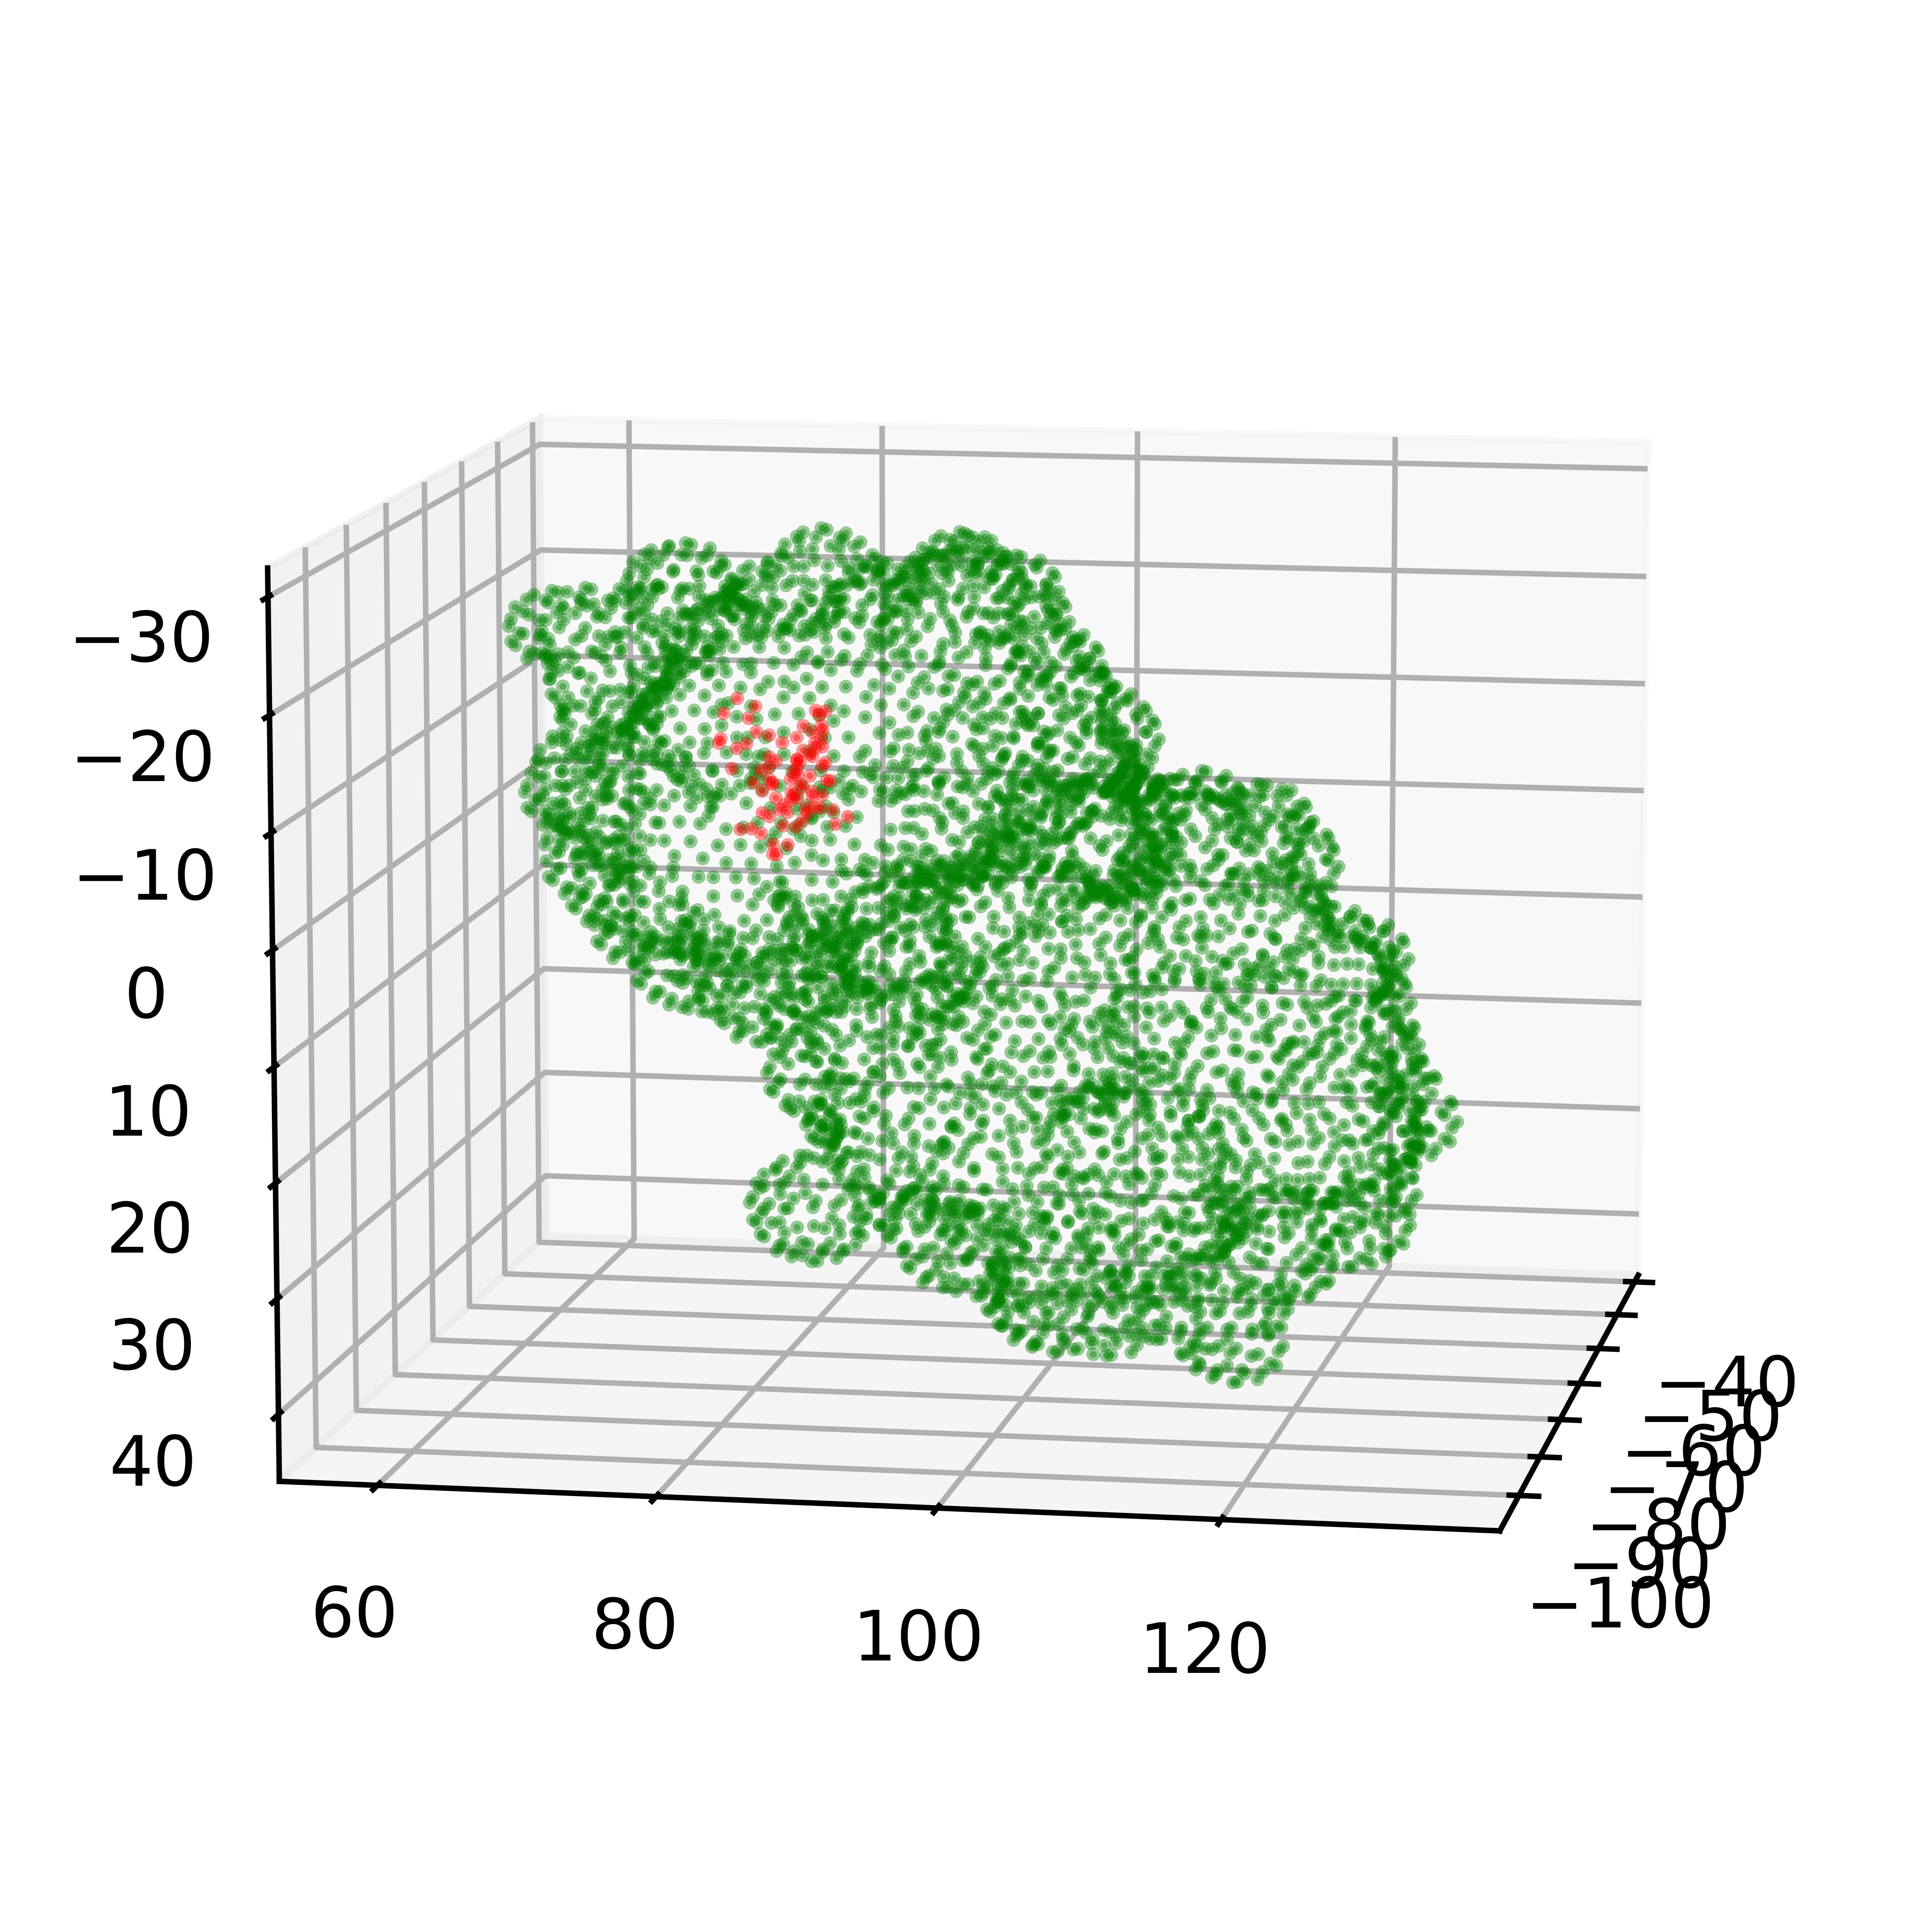
\includegraphics[width=1\linewidth]{point_cloud_class.png}
    \caption{SAS point cloud representing a protein with a highlighted ligand-binding site (in red). This point cloud is the input into the whole pipeline discussed in this work. Compare it to the P2Rank visualization in ~\ref{fig:p2rank_visualization} and feature visualization in 
    ~\ref{fig:pca_point_cloud}. This visualization was created by matplotlib.pyplot.scatter3D.}
    \label{fig:class_point_cloud}
\end{figure}

\begin{figure}
    \centering
    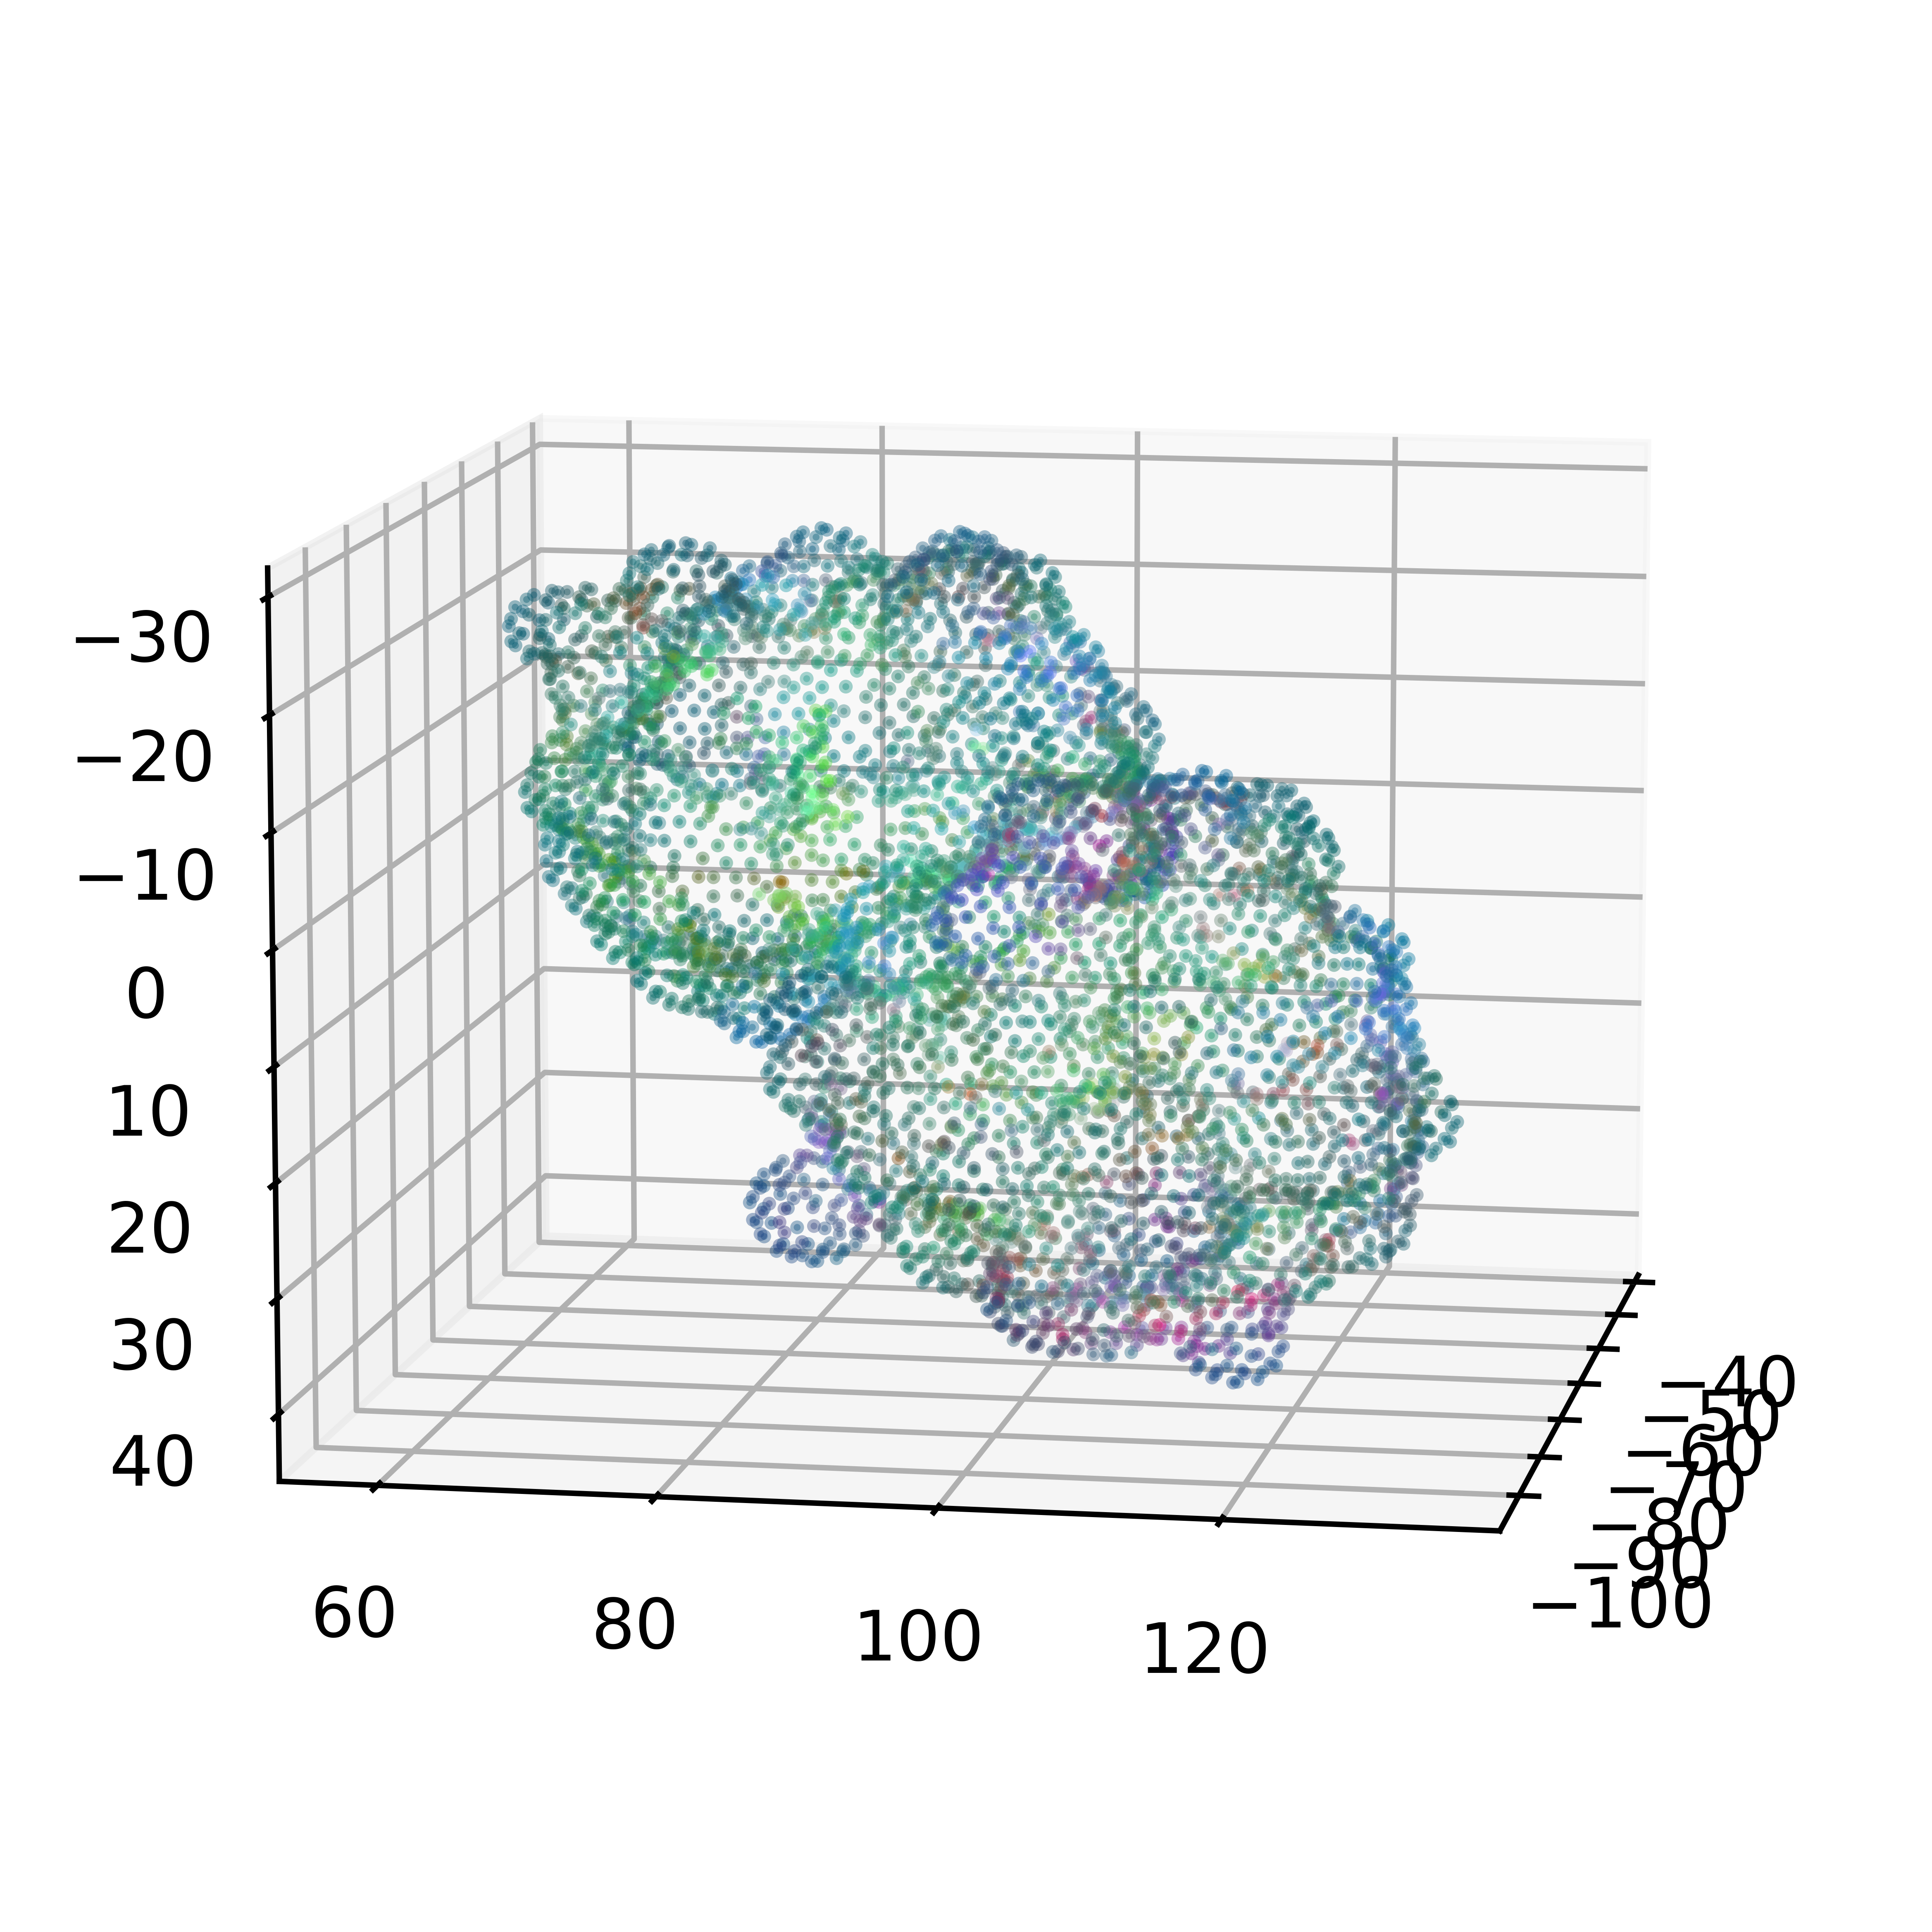
\includegraphics[width=1\linewidth]{point_cloud_pca.png}
    \caption{SAS point cloud showing the distribution of features across the surface. To achieve this visualization, locational and class-defining features were removed. Scikit-learn's PCA then reduced the remaining 35 dimensions to 3 dimensions. These were then plotted as red, green and blue channels using matplotlib.pyplot.scatter3D. It can be seen that there are no major feature outliers in the \ac{LBS} area.}
    \label{fig:pca_point_cloud}
\end{figure}

In the implementation, these points are represented as tabular data, with three columns representing the X, Y, and Z axis, respectively. From this data, the point cloud can be recreated.

\subsection{Ligand-binding sites}

In our data, clusters of points represent \ac{LBS}s). There is usually exactly one LBS per protein, but more can also exist. In some cases, no LBS is in the whole protein (but most of these proteins have been filtered out during the data preprocessing in the P2Rank dataset creation).

\subsection{Features}
\label{features_section}

As mentioned above, each point from the cloud has a feature vector attached (described in ~\ref{features_section}). These features are fully described in the following section. The exact features are essential for result reproducibility, however, they are not crucial for understanding these experiments. 

These features represent chemical properties of the protein surface (such as hydrophobicity), surface shape (protrusion), or physical properties (XYZ coordinates). All of them represent a float value and are used as such - no class features are used (atomic number could be seen as a class feature, but similarly sized atoms will have some similarities in their properties, so this feature is used as a numeric one). For the features list, see attachment ~\ref{feature_list}.

\subsection{Exact datasets}

Two datasets were used in this work, taken from the original P2Rank paper. First of them is \textbf{CHEN11}, a dataset of 251 proteins harboring 476 ligands introduced in \ac{LBS} prediction benchmarking study by \cite{chen11}. This dataset is used in the original paper as the training set and is used the same way in this work. A more detailed description is available in \cite{chen11}.

For model evaluation, the \textbf{COACH420} dataset is used. This dataset is shown in P2Rank as well. It is the test dataset from COACH(\cite{coach1}, \cite{coach2}), with all the proteins from the CHEN11 (and one other dataset from P2Rank) removed. 

\subsection{Surroundings extraction}
\label{Surroundings}

As described above, \ac{LBS} are represented by clusters of positively marked \ac{SAS} points. In P2Rank, features for all points are evaluated individually, but it makes sense that the surroundings of each SAS point influence whether a point is an LBS or not. To use this fact, the following algorithm to extract the surroundings is run (some parts were simplified compared to the actual code by omitting performance improvements and ignoring some syntactical parts for the reasons of readability):

\begin{lstlisting}
def extract_surroundings(protein: pd.DataFrame, size: int, labels: pd.Series) -> np.array:
  surroundings_dataset = []
  for i in range(len(protein)):
    surroundings_datasetFor.append(
      protein.sort(key = lambda x: mahattan_distance(i, x)
        )[:size].flatten()
      )
  return surroundings_dataset, labels
\end{lstlisting}

Or, in natural language, for each point in the original protein surface, the $k$ nearest points to the original point are used, and all features from these points are concatenated. Labels are kept from the original data.

Having a larger context naturally improves the performance of any model. In \cite{P2RANK}, proposing this dataset, a larger context area is not considered in the models themselves but as a postprocessing step, where clusters of positively predicted points are used for \ac{LBS} identification. For our use case, it also brings value in increasing the dimensionality of our data, allowing us to use image-based classifiers.

\section{Models}

Let's now look at the models. Each model should predict whether a given \ac{SAS} point is a part of an \ac{LBS}. The simplest model is the \textit{P2Rank RFC} model. This is an RFC-based classifier proposed in the original paper by \cite{P2RANK}, using only the single SAS point's features for prediction. Then, we have two more state-of-the-art baselines used on the surroundings dataset. These are \textit{RFC Surrounding}, which uses the same general algorithm of RFC prediction. Still, instead of using only the single point's features as the \textit{P2Rank RFC}, it uses the surroundings dataset. Similarly, the \textit{NN} model uses the same input as \textit{RFC Surrounding} but uses a dense neural network for the classification part. I then compare these to a set of CNN-based models, testing whether they can perform better than the more common, simpler models.

All models have their hyperparameter optimization described with them. \textbf{Highlighted} parts show the best value found in the first experiment (~\ref{first_experiment}).

\subsection{Model interface}

These models have a common interface of a method \texttt{predict(protein)}, which takes a protein as an input and returns the predicted probability of each input point being an \ac{LBS}. For better performance, if not specified otherwise, each model accepts the protein in the surroundings-based format described in \hyperref[Surroundings]{the corresponding section}. This way, the surroundings dataset can be cached, as the computation of it takes multiple hours.

\subsection{Baseline - P2Rank RFC}
As the first model, the original model from \cite{P2RANK} is recreated. This is the only model that takes the data in the original format. This is used as a baseline model to compare other models, with the one proposed in the original paper.

This model uses scikit-learn's RandomForestClassifier \ac{RFC} [\cite{scikit-learn}] as a predictor. As described in the original paper, it uses 200 trees with no depth limit and considers a maximum of 6 features in each split. The rest of the parameters are set to default values as described in the \hyperlink{https://scikit-learn.org/1.1/modules/generated/sklearn.ensemble.RandomForestClassifier.html}{corresponding documentation}. This is the simplest model for the job. It simply takes the features for each \ac{SAS} point and returns a probability of each point being in an \ac{LBS}.

With this model, no hyperparameter optimization was done. Instead, the parameters mentioned in P2Rank were used.

\subsection{Surrounding RFC}

Similarly to the Baseline RF model, this model uses an \ac{RFC} as the predictor. As with all the following models, this one is trained and used on the surroundings dataset. Hyperparameters were tuned using cross-validation on 5 splits, with exhaustive grid search from \cite{scikit-learn} and the target of minimizing the binary cross-entropy. Compared to the \textit{P2Rank RFC}, this model takes the features from the predicted point and all the features from the closest 30 points to it. This should allow the model to predict not only based on the wider chemical properties but also on physical factors, such as the shape of the surface. 

Hyperparameter optimization was done using cross-validation grid search with 5 cross-validation splits over the following grid space:
\begin{itemize}
    \item max-depth: [3, 5, \textbf{10}, None]
    \item min-samples-split: [2, \textbf{5}, 10]
    \item n-estimators: [100, 200, 300, \textbf{500}, 1000]
    \item max-features: [\textbf{sqrt}, log2, None]
\end{itemize}
For closer definitions, see scikit-learn documentation. All other parameters were kept on default scikit-learn values, except for allowing multithreading and controlling logging.

\subsection{NN}

Another common approach for classification is dense neural networks (NN). The model was optimized using Adam to minimize binary cross-entropy on a 1-unit, sigmoid-activated last layer. The exact architecture was created by hyperparameter tuning using the Hyperband tuner from the keras-tuner framework.
The hyperparameter space was the following:
\begin{itemize}
    \item learning-rate: [1e-2, 5e-3, 1e-3, \textbf{5e-4}, 1e-4, 5e-5]
    \item n-hidden-layers: 1 - 4 
    \item initial-hidden-layer: 16 - 4096
    \item growth-factor: 0.25 - 1.25
\end{itemize}

These set the learning rate and hidden layers (as the classification task and feature size give the input and output layers). The architecture has 1-4 hidden layers, where the first layer has \textit{initial-hidden-layer} neurons, and every following layer has the previous number of neurons multiplied by the \textit{growth-factor}.

\subsection{Random CNN}

For another baseline, I used the Random \ac{CNN} model. It transforms the input vector (same as with Surrounding RFC) into a matrix of $30 \times 38$ by randomly assigning features to positions. Then, a CNN is used as the predictor based on this created matrix. Hyperparameters are tuned only for the CNN (as there are no hyperparameters anywhere else). Keras-tuner Hyperband was used to find the best architecture following this structure (\textit{optimizable parameters highlighted by italics}):
\begin{itemize}
    \item InputLayer((38,30))
    \item \textit{Conv-layers} $\times$ Conv2D(filters=\textit{initial-size}*\textit{growth-factor}$^i$,\\
    \textit{stride}, \textit{kernel-size}, activation=ReLU)
    \item Flatten()
    \item Dense(\textit{last-dense}, activation=ReLU)
    \item Dense(1, activation=sigmoid)
\end{itemize}
Where the parameters are from the following ranges:
\begin{itemize}
    \item \textit{learning-rate}: [1e-2, 5e-3, 1e-3, 5e-4, 1e-4, 5e-5]
    \item \textit{Conv-layers}: 1 - 4
    \item \textit{initial-size}: 16 - 4096
    \item \textit{growth-factor}: 0.25 - 1.5
    \item \textit{stride}: 1 - 3
    \item \textit{kernel-size}: 3 - 7
    \item \textit{last-dense}: 16 - 4096
\end{itemize}

The model was then trained using the Adam optimizer to minimize the binary cross-entropy loss. 

\subsection{Normalized CNN}

This is a variation on Random \ac{CNN}, where each feature is first normalized to follow $N(0, 1)$. This should simulate an image more closely, where the pixels are also all bound by some distribution (mainly bound by being between 0 and 1). The rest of the model is the same as \textit{Random CNN} (reshaping into a matrix, same CNN architecture with the same hyperparameter optimization).

\subsection{REFINED}

This model is a continuation of the previous model. The only difference is that, instead of randomly distributing features in the matrix, REFINED moves the features around to achieve a more controlled distribution of features in the final image. It streamlines an approach proposed by \cite{REFINED}. Compared to the original approach, the DR preprocessing step is skipped. The whole algorithm is simplified in the following list. 

\begin{enumerate}
    \item Input: Set of samples $X = x_1, ... x_n$, where $\forall i x_i \in \mathbb{R}^{D}$, where $D$ is the number of features for each sample (in this case feature vector as described in \hyperref[Surroundings]{the surroundings extraction section}.
    \item Each feature is regularized to follow $f \sim N(0,1)$
    \item Each sample is reshaped to $x_i \in R^{k\times l}$, where $k\cdot l = D$.
    \item Features are reordered in the images to create gradients (see ~\ref{REFINED_core} for more details).
    \item Using this permutation, a matrix is created for each sample used in the following step.
    \item A \ac{CNN} classifier is trained on the provided data.
\end{enumerate}

\subsubsection{Pre-REFINED preprocessing}

The first step in the REFINED pipeline is data normalization. For each feature, the mean and standard deviation is calculated. Then, the mean is subtracted from each feature value and divided by the standard deviation. With normally distributed features, this will produce a feature following the $N(0,1)$ normal distribution. For other features, this will give us a distribution where $\mu=0$ and $\sigma=1$. 

In the original paper, the data normalization step is omitted because DR techniques stand in its place, all of which in some way provide data normalization. Non-normalized data made results from REFINED core visually worse than normalized ones. After explaining the relevant context, I'll discuss why this is the case in the REFINED core and \ac{CNN} sections.

After normalization, features are randomly assigned to the locations in the resulting matrix. Random allocation is used instead of simple row wrapping (having the features sustain the same order, just wrapped to form a matrix) because the core algorithm might get stuck in a local minimum caused by the initial feature distribution. This was the case, especially with the used dataset, because features from neighboring points are often strongly correlated. This was seen in the images produced by the REFINED core, which were close to the original ones.

\subsubsection{REFINED core}
\label{REFINED_core}
Now comes the exciting part of the algorithm.  To allow the location of the feature in the image to have some meaning, the REFINED score is minimized over all the permutations of features ($P([D])$): 
    $$ f(O|X) = \sum_{s=1}^{n} \sum_{i, j, k, l =1}^n (x^O_{s, ij} - x^O_{s, kl})^2 \cdot \abs{[i,j] - [k,l]}^{-1}$$
Where
\begin{itemize}
    \item $f(O|X): P([D]) \rightarrow \mathbb{R}$ is the REFINED score,
    \item $O \in P([D])$ is an ordering of the features
    \item $x^O_s$ is the sample $x_s$ ordered by the ordering $O$
\end{itemize}
Then $x^O_{s, ij}$ is the value is sample $x_s$ on matrix index $[i,j]$ given that the features are ordered by the ordering $O$.

As this is computationally an exponential problem, this optimum is approximated using the hill climbing algorithm (HCA) \footnote{\label{hca_description}HCA is an algorithm that starts with an arbitrary solution (in our case, a random feature allocation strategy) and then at every step tries to find a better solution (a permutation with a lower REFINED score) making and incremental step (switching the places of 2 neighboring features in our case). If no step will improve the solution, it finishes. It is not guaranteed to find the optimal permutation, as it can end in a local minimum.}. Even though this algorithm isn't guaranteed to find the optimal solution, it is used here, as there isn't a technologically viable solution to find the global minimum. This method was also used in the original REFINED paper and is reused in this work.

HCA requires not only the value function $f(X|O)$ but also the neighborhood function $h(O): P([D]) \rightarrow X \in \mathcal{P}(P([D]))$ (output is a subset of $P([D])$ - or a list of orderings). This can be easily computed with the following algorithm:
\begin{lstlisting}
def h(ordering:np.ndarray) -> List[np.ndarray]:
  ret = []
  for i in range(ordering.shape[0]):
    for j in range(ordering.shape[1]):
      for (k, l) in neighboring_pixels(i,j):
        ret.append(swapped(ordering, (i, j), (k, l)))
  return ret

def swapped(array: np.ndarray,
        index0: Tuple[int, int],
        index1: Tuple[int, int]) -> np.ndarray:
    array[index0], array[index1] = array[index1], array[index0]
    return array

def neighboring_pixels(x: int, y: int) -> List[Tuple[int, int]]:
    return [(x + dx, y + dy) 
              for dx in (-1, 0, 1)
              for dy in (-1, 0, 1)
              if (0 <= x + dx < k and 0 <= y + dy < l)
                or not (dx == dy == 0)
            ]
\end{lstlisting}

For complexity's sake, all the neighbors aren't calculated together for the whole ordering, but after each pixel's neighbors are calculated (so for each $i,j$ from the code), the ordering with the lowest value function is greedily chosen (or keep the original one, if it is the best) and all the remaining neighbors are calculated from this modified state. This increases performance for as many as $D$ steps per calculation of value functions for the whole ordering neighborhood can be taken. However, as it follows the value function's gradient more approximately, it could lead to a higher chance of ending up at a local minimum. Still, this algorithm runs for multiple hours as is, and this can be partly avoided by running multiple HCA's in parallel.

For this work, I used my own Python implementation of HCA to ensure a smoother integration into the rest of the pipeline. To make this implementation run faster, Numba JIT was used on the most performance-critical methods. Combined with the greedy computation described in the previous paragraph, finishing the entire REFINED core run takes only a few hours.

This algorithm creates a feature ordering with correlated features near each other in a generated image and negatively correlated features further away. In Figure ~\ref{fig:REFINED_visualized} the process of how features move can be seen. This can make it easier for humans to see differences between samples compared to looking at the data simply as a vector.

In one of the first experiments, I tried using a genetic evolutionary algorithm (\ac{GEA}), but it proved to be much slower than the simple HCA - at least with the configuration used then. HCA can be further optimized and run multiple times in parallel, avoiding its pitfalls (getting stuck in a local minimum). Although I didn't succeed with GEA in this part of the algorithm, with some additional work, it might be faster. But this is out of the scope of this work.

As foreshadowed earlier, the REFINED core does not work well with non-normalized data. This can be easily explained. The REFINED core works by aligning correlated features together. However, to make the process easier, only the $L2$ norm of the difference between each feature is computed. This causes features with different means to be further away from each other. Not only that, it causes features with higher variations to be further away from each other. Small differences between low-variational features then influence the value function very little compared to high-variational features with vastly different means. However, this information is not useful for the predictor following this step.

\section{Evaluation Criteria}

Every method was evaluated using some performance criteria. In the following part, I will describe these metrics.

Because all used datasets are imbalanced (97 \% of samples are negative), the $F_1$-score is used as the main evaluation metric. However, accuracy, precision, and recall are all calculated. Given that $TP$ is the number of true positives, $FP$ false positives, $TN$ true negatives and $FN$ false positives, aforementioned metrics are defined as follows:
$$F_1 = \frac{2TP}{2TP + FP + FN}$$
$$Accuracy = \frac{TP + TN}{TP + FP + TN + FN}$$
$$Precision = \frac{TP}{TP + FP}$$
$$Recall = \frac{TP}{TP + FN}$$

In order to obtain the variance between different runs of the same model architecture, 5 models are trained for each architecture in a cross-validation-like pattern (always using $\frac{4}{5}$ of the training dataset). For a more precise description, see section ~\ref{experiments}.